\documentclass[stat333]{subfiles}

%% ========================================================
%% document

\begin{document}

    \chap{Markov Chains}

    \section{Markov Chains}

    \begin{definition}{Stochastic Process}{}
        Any collection of random variables (or random vectors) of the form $\left\lbrace X\left( t \right) \right\rbrace^{}_{t\in\mT}$ is called a \emph{stochastic process}.
    \end{definition}

    \np Given a stochastic process $\left\lbrace X\left( t \right) \right\rbrace^{}_{t\in\mT}$ The index set $\mT$ is often interpreted in the context of time. As such, usually $\mT\subseteq\R$ and we say $X\left( t \right)$ is the \emph{state} of the process at time $t\in\mT$.

    \begin{definition}{Continuous-time, Discrete-time}{Stochastic Process}
        Let $\left\lbrace X\left( t \right) \right\rbrace^{}_{t\in\mT}$ be a stochastic process. We say $\left\lbrace X \right\rbrace^{}_{t\in\mT}$ is 
        \begin{enumerate}
            \item \emph{continuous-time} if $\mT$ is a (union of) continuum of real numbers; and
            \item \emph{discrete-time} if $\mT$ is a countable subset of real numbers.\footnote{In general, we use $\N\cup\left\lbrace 0 \right\rbrace$ as the index set of discrete-time stochastic processes. In fact, we shall use this convention throughout this note, unless otherwise specified.}
        \end{enumerate}
    \end{definition}

    \begin{definition}{Discrete-time Markov Chain (DTMC)}{}
        We say a discrete-time stochastic process $\left\lbrace X_n \right\rbrace^{}_{n\in\N\cup\left\lbrace 0 \right\rbrace}$ is a \emph{discrete-time Markov chain} (\emph{DTMC}) if
        \begin{enumerate}
            \item each $X_n$ is discrete; and
            \item for every $n\in\N\cup\left\lbrace 0 \right\rbrace$ and $x_0,\ldots,x_{n+1}$ in the codomain of $X_0,\ldots,X_{n+1}$, respectively,
                \begin{equation*}
                    \PP\left( X_{n+1}=x_{n+1}|X_{n}=x_{n},\ldots,X_0=x_0 \right) = \PP\left( X_{n+1}=x_{n+1}|X_{n}=x_{n} \right).\eqno\text{\textit{Markov property}}
                \end{equation*}
        \end{enumerate}
    \end{definition}

    \np In other words, the Markov property states that the conditional distribution of a \textit{future} state $X_{n+1}$ given the \textit{past} states $X_0,\ldots,X_{n-1}$ and the \textit{present} state $X_n$ is independent of the past states. It is also worth noting that the Markov property ensures that, given any $k_1,\ldots,k_l\in\left\lbrace 1,\ldots,n-1 \right\rbrace$ with $k_1<\cdots<k_l$,
    \begin{equation*}
        \PP\left( X_{n+1}=x_{n+1}|X_{k_l}=x_{k_l},\ldots,X_{k_1}=x_{k_1} \right) = \PP\left( X_{n+1}=x_{n+1}|X_{k_l}=x_{k_l} \right).
    \end{equation*}

    \begin{definition}{Transition Probability Matrix}{}
        For any pair of states $i,j\in\N\cup\left\lbrace 0 \right\rbrace$, the \emph{transition probability} from state $i$ at time $n$ to state $j$ at time $n+1$ is given by
        \begin{equation*}
            \PP\left( X_{n+1}=j|X_n=i \right)
        \end{equation*}
        for all $n\in\N\cup\left\lbrace 0 \right\rbrace$. The \emph{transition probability matrix} from time $n$ to time $n+1$ is defined as 
        \begin{equation*}
            \begin{bmatrix}
                P_{n,0,0} & P_{n,0,1} & \cdots \\
                P_{n,1,0} & P_{n,1,1} & \cdots \\
            	\vdots & \vdots & \ddots \\
            \end{bmatrix}
        \end{equation*}
        for all $n\in\N\cup\left\lbrace 0 \right\rbrace$, where $P_{n,i,j}=\PP\left( X_{n+1}=j|X_n=i \right)$ for all $i,j\in\N\cup\left\lbrace 0 \right\rbrace$.
    \end{definition}

    \clearpage
    \np It is clear from the construction that, given any TPM $P$,
    \begin{enumerate}
        \item every entry of $P$ is nonnegative; and
        \item for any row of $P$, the sum of the entries is $1$.
    \end{enumerate}
    Any matrix that satisfies (a), (b) is called \emph{stochastic}.

    \begin{definition}{Stationary (Homogeneous)}{DTMC}
        Let $\left\lbrace X_n \right\rbrace^{}_{n\in\N\cup\left\lbrace 0 \right\rbrace}$ be a DTMC. We say $\left\lbrace X_n \right\rbrace^{}_{n\in\N\cup\left\lbrace 0 \right\rbrace}$ is \emph{stationary} (or \emph{homogeneous}) if the transition probability is independent of the time.\footnote{We shall only consider stationary DTMCs in this note.} That is, for all times $n,m\in\N\cup\left\lbrace 0 \right\rbrace$ and indices $i,j\in\N\cup\left\lbrace 0 \right\rbrace$,
        \begin{equation*}
            \PP\left( X_{n+1}=j|X_n=i \right) = \PP\left( X_{m+1}=j|X_n=i \right).
        \end{equation*}
    \end{definition}


    \ex On a given day the weather is clear, overcast, or rainy. 
    If the weather is clear today, then it would be clear, overcast, or rainy tomorrow with respective probabilities $0.6,0.3,0.1$. 
    If the weather is overcast today, then it would be clear, overcast, or rainy tomorrow with respective probabilities $0.2,0.5,0.3$. 
    If the weather is rainy today, then it would be clear, overcast, or rainy tomorrow with respective probabilities $0.4,0.2,0,4$. 
    Construct the underlying DTMC and determine its TPM.

    \begin{subproof}[Answer]
        Note that the weather tomorrow only depends on the weather today, implying that the Markov property holds. Hence, letting
        \begin{equation*}
            X_n = 
            \begin{cases} 
                0 & \text{if the weather on $n$th day is clear}\\
                1 & \text{if the weather on $n$th day is overcast}\\
                2 & \text{if the weather on $n$th day is rainy}
            \end{cases},
        \end{equation*}
        $\left( X_{n} \right)^{}_{n\in\N\cup\left\lbrace 0 \right\rbrace}$ is a $3$-state DTMC. Moreover, the TPM is given by
        \begin{equation*}
            \begin{bmatrix}
            	0.6 & 0.3 & 0.1 \\
            	0.2 & 0.5 & 0.3 \\
            	0.4 & 0.2 & 0.4 \\
            \end{bmatrix}. \eqqedsym
        \end{equation*}
    \end{subproof}

    \begin{definition}{$n$-step Transition Probability}{}
        Suppose that we have a DTMC $\left\lbrace X_n \right\rbrace^{}_{n\in\N\cup\left\lbrace 0 \right\rbrace}$. For every states $i,j\in\N\cup\left\lbrace 0 \right\rbrace$ and $n\in\N\cup\left\lbrace 0 \right\rbrace$, we define the \emph{$n$-step transition probability}, commonly denoted as $P^{\left( n \right)}_{i,j}$, as
        \begin{equation*}
            P^{\left( n \right)}_{i,j} = \PP\left( X_{m+n}=j|X_m=i \right),
        \end{equation*}
        where $m\in\N\cup\left\lbrace 0 \right\rbrace$.\footnote{The definition is independent of $m$ since we assumed our DTMC to be stationary. In other words, we may define $P^{\left( n \right)}_{i,j}=\PP\left( X_n=j|X_0=i \right)$.} We call
        \begin{equation*}
            P^{\left( n \right)} = \left[ P^{\left( n \right)}_{i,j} \right]_{i,j\in\N\cup\left\lbrace 0 \right\rbrace}
        \end{equation*}
        the \emph{$n$-step transition probability matrix} (\emph{$n$-step TPM}).
    \end{definition}

    \clearpage
    \np Consider a DTMC $\left\lbrace X_n \right\rbrace^{}_{n\in\N\cup\left\lbrace 0 \right\rbrace}$, its TPM $P$, and $n$-step TPMs $P^{\left( 0 \right)}, \ldots$.
    \begin{enumerate}
        \item From the construction, it is evident that
            \begin{equation*}
                P^{\left( 0 \right)}_{i,j}=\delta_{ij}
            \end{equation*}
            for every states $i,j$, where $\delta$ is the Kronecker delta. It follows that $P^{\left( 0 \right)}$ is the identity matrix.
        \item $P^{\left( 1 \right)}=P$.
    \end{enumerate}
    
    \np[Chapman-Kolmogorov Equations]For any $n\in\N$, we have
    \begin{equation}
        P^{\left( n \right)}_{i,j} = \sum^{\infty}_{k=0}P^{\left( n-1 \right)}_{i,k}P_{k,j}.
    \end{equation}

    \begin{subproof}
        Observe that    
        \begin{flalign*}
            && P^{\left( n \right)}_{i,j} & = \PP\left( X_n=j|X_0=i \right) && \\ 
            && & = \sum^{\infty}_{k=0}\PP\left( X_n=j|X_{n-1}=k,x_0=i \right)\PP\left( X_{n-1}=k|X_0=i \right) && \\
            && & = \sum^{\infty}_{k=0}P^{\left( n-1 \right)}_{i,k}\PP\left( X_n=j|X_{n-1}=k,X_0=i \right) && \\
            && & = \sum^{\infty}_{k=0}P^{\left( n-1 \right)}_{i,k}\PP\left( X_n=j|X_{n-1}=k \right) && \text{by Markov property}\\
            && & = \sum^{\infty}_{k=0}P^{\left( n-1 \right)}_{i,k}P_{k,j}, 
        \end{flalign*} 
        as required.
    \end{subproof}
    
    \noindent This in particular implies that,
    \begin{equation}
        P^{\left( n \right)} = P^{\left( n-1 \right)}P
    \end{equation}
    for every $n\in\N$, and as a corollary,
    \begin{eqbox}[Chapman-Komogorov Equations for a DTMC]
        \begin{equation}
            P^{\left( n \right)}_{i,j} = \sum^{\infty}_{k=0}P^{\left( m \right)}_{i,k}P^{\left( n-m \right)}_{k,j}
        \end{equation}
    \end{eqbox} 
    for every $i,j\in\N\cup\left\lbrace 0 \right\rbrace$ and $n\in\N, m\in\left\lbrace 0,\ldots,n \right\rbrace$. In matrix form, this translates to
    \begin{eqbox}[Chapman-Komogorov Equations in Matrix Form]
        \begin{equation}
            P^{\left( n \right)} = P^{\left( m \right)}P^{\left( n-m \right)}.
        \end{equation}
    \end{eqbox} 

    \np Consider the row vector
    \begin{equation*}
        \alpha_n = \begin{bmatrix} \alpha_{n,0} & \alpha_{n,1} & \cdots  \end{bmatrix}
    \end{equation*}
    for every $n\in\N\cup\left\lbrace 0 \right\rbrace$, where
    \begin{equation*}
        \alpha_{n,k} = \PP\left( X_n=k \right)
    \end{equation*}
    for every $k\in\N$. In other words, $\alpha_n$ represents the marginal pmf of $X_n$, and as a consequence,
    \begin{equation*}
        \sum^{\infty}_{k=0}\alpha_{n,k} = 1.
    \end{equation*}
    In case $n=0$, $\alpha_0$ is referred to as the \emph{initial conditions} (or \emph{initial probability row vector}) of the DTMC. Now let us see how we can calculate $\alpha_n$. For every $n\in\N, m\in\left\lbrace 0,\ldots,n \right\rbrace$, note that
    \begin{flalign*}
        && \alpha_{n,k} & = \PP\left( X_n=k \right) && \\ 
        && & = \sum^{\infty}_{i=0}\PP\left( X_n=k|X_m=i \right)\PP\left( X_m=i \right) && \\
        && & = \sum^{\infty}_{i=0}\alpha_{m,i}\PP\left( X_{n-m}=k|X_0=i \right) && \text{since the DTMC is stationary} \\
        && & = \sum^{\infty}_{i=0}\alpha_{m,i}P_{i,k}^{\left( n-m \right)}.
    \end{flalign*} 
    In matrix form,
    \begin{equation*}
        \alpha_n = \alpha_mP^{\left( n-m \right)} = \alpha_mP^{n-m},
    \end{equation*}
    or
    \begin{eqbox}[Marginal PDF of $X_n$]
        \begin{equation}
            \alpha_n = \alpha_0P^n.
        \end{equation}
    \end{eqbox} 

    \np Having knowledge of the initial conditions and the one-step transition probabilities, one can calculate various probabilites of possible interest, such as
    \begin{flalign*}
        && \PP\left( X_n=x_n, \ldots, X_0=x_0 \right)& = \PP\left( X_0=x_0 \right)\PP\left( X_1=x_1|X_0=x_0 \right)\cdots\PP\left( X_n=x_n|X_{n-1}=x_{n-1},\ldots,X_0=x_0 \right) && \\ 
        && & = \PP\left( X_0=x_0 \right)\PP\left( X_1=x_1|X_0=x_0 \right)\cdots\PP\left( X_n=x_n|X_{n-1}=x_{n-1} \right) && \\
        && & = \alpha_{0,x_0}P_{x_0,x_1}\cdots P_{x_{n-1},x_n}. 
    \end{flalign*} 
    Similarly,
    \begin{flalign*}
        && & \PP\left( X_{n+m}=x_{n+m},\ldots,X_{n+1}=x_{n+1}|X_n=x_n \right) && \\
        && & = \frac{\PP\left( X_{n+m}=x_{n+m},\ldots,X_n=x_n \right)}{\PP\left( X_n=x_n \right)} && \\ 
        && & = \frac{\PP\left( X_n=x_n \right)\PP\left( X_{n+1}=x_{n+1}|X_n=x_n \right)\cdots\PP\left( X_{n+m}=x_{n+m}|X_{n+m-1}=x_{n+m-1},\ldots,X_n=x_n \right)}{\PP\left( X_n=x_n \right)} && \\
        && & = P_{x_n,x_{n+1}}\cdots P_{x_{n+m-1},x_{n+m}}.
    \end{flalign*} 
    The key observation is that the DTMC is \textit{completely characterized} by its one-step TPM $P$ and the initial conditions $\alpha_0$.
    
    \ex A particle moves along the states $0,1,2$ according to a DTMC whose TPM $P$ is given by
    \begin{equation*}
        P = 
        \begin{bmatrix}
        	0.7 & 0.2 & 0.1 \\
        	0 & 0.6 & 0.4 \\
        	0.5 & 0 & 0.5 \\
        \end{bmatrix}.
    \end{equation*}
    Let $X_n$ denote the position of the particle after the $n$th move (i.e. the DTMC is $\left\lbrace X_n \right\rbrace^{}_{n\in\N\cup\left\lbrace 0 \right\rbrace}$). Suppose that the particle is equally likely to start in any of the three positions.
    \begin{enumerate}
        \item Calculate $\PP\left( X_3=1|X_0=0 \right)$.

            \begin{subproof}[Answer]
                We desire to find $P_{0,1}^{\left( 3 \right)}$. To get this, we proceed to calculate $P^{\left( 3 \right)}$, the $3$-step transition TPM, which satisfies
                \begin{equation*}
                    P^{\left( 3 \right)} = P^3
                \end{equation*}
                where $P$ is the TPM. First of all,
                \begin{equation*}
                    P^2 = 
                    \begin{bmatrix}
                    	0.54 & 0.26 & 0.2 \\
                    	0.2 & 0.36 & 0.44 \\
                    	0.6 & 0.1 & 0.3 \\
                    \end{bmatrix}
                \end{equation*}
                and
                \begin{equation*}
                    P^3 = 
                    \begin{bmatrix}
                    	0.478 & 0.264 & 0.258 \\
                    	0.36 & 0.256 & 0.384 \\
                    	0.57 & 0.18 & 0.25 \\
                    \end{bmatrix}
                \end{equation*}
                by direct calculations. Thus,
                \begin{equation*}
                    P_{0,1}^{\left( 3 \right)} = P_{0,1}^3 = 0.264. \eqqedsym
                \end{equation*}
            \end{subproof}

        \item Calculate $\PP\left( X_4=2 \right)$.

            \begin{subproof}[Answer]
                We desire to find
                \begin{equation*}
                    \alpha_{4,2} = \PP\left( X_4=2 \right).
                \end{equation*}
                To do so, let us calculate $\alpha_4$, which satisfies
                \begin{equation*}
                    \alpha_4 = \alpha_0P^4.
                \end{equation*}
                By a direct calculation,
                \begin{equation*}
                    P^4 = 
                    \begin{bmatrix}
                    	\frac{1159}{2500} & \frac{127}{500} & \frac{353}{1250} \\
                    	\frac{111}{250} & \frac{141}{625} & \frac{413}{1250} \\
                    	\frac{131}{250} & \frac{111}{500} & \frac{127}{500} \\
                    \end{bmatrix},
                \end{equation*}
                so
                \begin{equation*}
                    \alpha_4 = \alpha_0P^4 = \begin{bmatrix} \frac{1}{3} & \frac{1}{3} & \frac{1}{3} \end{bmatrix}
                    \begin{bmatrix}
                    	\frac{1159}{2500} & \frac{127}{500} & \frac{353}{1250} \\
                    	\frac{111}{250} & \frac{141}{625} & \frac{413}{1250} \\
                    	\frac{131}{250} & \frac{111}{500} & \frac{127}{500} \\
                    \end{bmatrix}
                    =
                    \begin{bmatrix} \frac{1193}{2500} & \frac{877}{3750} & \frac{2167}{7500} \end{bmatrix}.
                \end{equation*}
                Thus
                \begin{equation*}
                    \alpha_{4,2} = \frac{2167}{7500}. \eqqedsym
                \end{equation*}
            \end{subproof}

        \item Calculate $\PP\left( X_6=0, X_4=2 \right)$.

            \begin{subproof}[Answer]
                We have
                \begin{equation*}
                    \PP\left( X_6=0, X_4=2 \right) = \PP\left( X_4=2 \right)\PP\left( X_6=0|X_4=2 \right) = \alpha_{4,2}P^{\left( 2 \right)}_{2,0} = 0.17336. \eqqedsym
                \end{equation*}
            \end{subproof}

        \item Calculate $\PP\left( X_9=0, X_7=2|X_5=1, X_2=0 \right)$.

            \begin{subproof}[Answer]
                We have
                \begin{flalign*}
                    && & \PP\left( X_9=0, X_7=2|X_5=1, X_2=0 \right) && \\
                    && & = \PP\left( X_7=2|X_5=1,X_4=0 \right)\PP\left( X_9=0|X_7=2,X_5=1,X_2=0 \right)  && \\
                    && & = \PP\left( X_7=2|X_5=1 \right)\PP\left( X_9=0|X_7=2 \right) = P^{\left( 2 \right)}_{1,2}P^{\left( 2 \right)}_{2,0} = 0.264.&&\fqqedsym
                \end{flalign*} 
            \end{subproof}
    \end{enumerate}

    \section{Accessibility and Communication}
    
    \begin{definition}{Accessble}{State}
        Let $i,j$ be states of a DTMC with $n$-step TPMs $P^{\left( n \right)}$.
        \begin{enumerate}
            \item We say $j$ is \emph{accessible} from state $i$, denoted as $i\to j$, if there exists $n\in\N\cup\left\lbrace 0 \right\rbrace$ such that $P^{\left( n \right)}_{i,j}>0$.
            \item We say $i,j$ \emph{communicate}, denoted as $i\lra j$ if $i\to j, j\to i$.
        \end{enumerate}
    \end{definition}

    \np In terms of accessibility, note that the magnitude of the components of $P$ do not matter. All that matters is which are positive and which are $0$. In particular, if state $j$ is not accessible from state $i$, then $P^{\left( n \right)}_{i,j} = 0$ for every $n\in\N\cup\left\lbrace 0 \right\rbrace$, and
    \begin{flalign*}
        && \PP\left( \exists m\in\N\cup\left\lbrace 0 \right\rbrace\left[ X_m = j \right]|X_0=i \right) & = \PP\left( \bigcup_{n\in\N\cup\left\lbrace 0 \right\rbrace}\left\lbrace X_n=j \right\rbrace|X_0=i \right) && \\ 
        && & \leq \sum^{\infty}_{n=0}\PP\left( X_n=j|X_0=i \right) = \sum^{\infty}_{n=0}P^{\left( n \right)}_{i,j} = 0.
    \end{flalign*} 
    In other words, if $j$ is not accessible from $i$, then the probability that the DTMC ever visits state $j$ given $X_0=i$ is $0$.

    \np Communication is an \textit{equivalence relation}. That is, given any states $i,j,k$, 
    \begin{enumerate}
        \item $i\lra i$;\hfill\textit{reflexivity}
        \item $i\lra j$ implies $j\lra i$; and\hfill\textit{symmetry}
        \item $i\lra j, j\lra k$ implies $i\lra k$.\hfill\textit{transitivity}
    \end{enumerate}

    \begin{subproof}
        (a), (b) are clear. To show transitivity, we know that there are $n,m\in\N\cup\left\lbrace 0 \right\rbrace$ such that $P^{\left( n \right)}_{i,j},P^{\left( m \right)}_{j,k}>0$. Then by the Chapman-Kolmogorov equations,
        \begin{equation*}
            P_{i,k}^{\left( n+m \right)} = \sum^{\infty}_{l=0}P_{i,l}^{\left( n \right)}P_{l,k}^{\left( m \right)}\geq P_{i,j}^{\left( n \right)}P_{j,k}^{\left( m \right)}>0.
        \end{equation*}
        Hence $i\to k$. Using the same logic, $k\to i$. Thus $i\lra k$.
    \end{subproof}

    \noindent The fact that communication forms an equivalence relation allows us to \textit{partition} all the states of a DTMC into equivalence classes, called \emph{communication classes}, so that within each class, all states communicate. For any states $i,j$ belong to distinct classes, \textit{at most} one of $i\to j, j\to i$ holds.

    \begin{definition}{Irreducible, Reducible}{DTMC}
        A DTMC is called
        \begin{enumerate}
            \item \emph{irreducible} if it has only one communcation class; and
            \item \emph{reducible} if not irreducible.
        \end{enumerate}
    \end{definition}

    \ex Suppose that the TPM $P$ of a DTMC is
    \begin{equation*}
        P = \left[ P_{i,j} \right]^{2}_{i,j=0}
        \begin{bmatrix}
        	0.7 & 0.2 & 0.1 \\
        	0 & 0.6 & 0.4 \\
        	0.5 & 0 & 0.5 \\
        \end{bmatrix}.
    \end{equation*}
    Find the communication classes of the DTMC.

    \begin{subproof}[Answer]
        We are going to draw a \textit{state transition diagram}.
        \begin{center}
            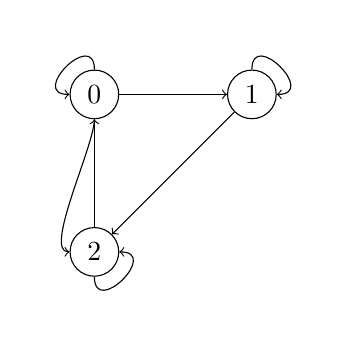
\begin{tikzpicture}[main/.style={draw,circle},node distance={2cm}]
                \node[main](0){$0$};
                \node[main](1)[right of=0]{$1$};
                \node[main](2)[below of=0]{$2$};
                \draw[->](0) to [out=90,in=180,looseness=3] (0);
                \draw[->](0) -- (1);
                \draw[->](0) to [out=270,in=180,looseness=0.5] (2);
                \draw[->](1) to [out=90,in=0,looseness=3] (1);
                \draw[->](1) -- (2);
                \draw[->](2) to [out=270,in=0,looseness=3] (2);
                \draw[->](2) -- (0);
            \end{tikzpicture}
        \end{center}
        Thus $\left\lbrace 0,1,2 \right\rbrace$ is the only communication class of the DTMC; in other words, the DTMC is irreducible.
    \end{subproof}

    \ex Consider a DTMC with TPM
    \begin{equation*}
        P =
        \begin{bmatrix}
        	0 & 1 & 0 & 0 \\
        	0 & 0 & 1 & 0 \\
        	0 & 0 & 0 & 1 \\
        	\frac{1}{2} & 0 & \frac{1}{2} & 0 \\
        \end{bmatrix}.
    \end{equation*}
    Find the communication classes of this DTMC.

    \begin{subproof}[Answer]
        By drawing a state transition diagram, it is clear that the DTMC is irreducible.
    \end{subproof}

    \ex Consider a DTMC with TPM
    \begin{equation*}
        P =
        \begin{bmatrix}
        	\frac{1}{3} & \frac{2}{3} & 0 & 0 \\
        	\frac{1}{2} & \frac{1}{4} & \frac{1}{8} & \frac{1}{8} \\
        	0 & 0 & 1 & 0 \\
        	\frac{3}{4} & \frac{1}{4} & 0 & 0 \\
        \end{bmatrix}.
    \end{equation*}
    Find the communication classes of this DTMC.

    \begin{subproof}[Answer]
        Observe that the state transition diagram is
        \begin{center}
            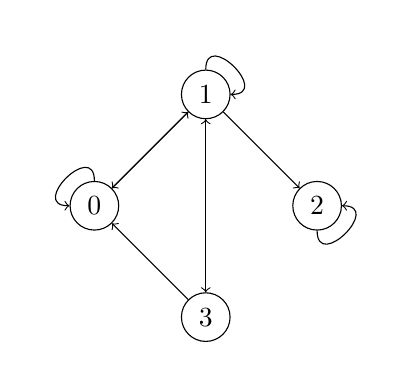
\begin{tikzpicture}[main/.style={draw,circle},node distance={2cm}]
                \node[main](0){$0$};
                \node[main](1)[above right of=0]{$1$};
                \node[main](2)[below right of=1]{$2$};
                \node[main](3)[below right of=0]{$3$};
                \draw[->](0) to [out=90,in=180,looseness=3] (0);
                \draw[->](0) -- (1);
                \draw[->](1) to [out=90,in=0,looseness=3] (1);
                \draw[->](1) -- (0);
                \draw[->](1) -- (2);
                \draw[->](1) -- (3);
                \draw[->](2) to [out=270,in=0,looseness=3] (2);
                \draw[->](3) -- (0);
                \draw[->](3) -- (1);
            \end{tikzpicture}
        \end{center}
        Thus $\left\lbrace 0,1,3 \right\rbrace, \left\lbrace 2 \right\rbrace$ are the communication classes of the DTMC.
    \end{subproof}

    \clearpage
    \section{Periodicity}
    
    \begin{definition}{Period}{of a State of a DTMC}
        Let $P$ be the TPM of a DTMC. Given a state $i$ of the DTMC, we define the \emph{period} of $i$, denoted as $d\left( i \right)$, by
        \begin{equation*}
            d\left( i \right) = 
            \begin{cases} 
                \gcd\left\lbrace n\in\N: P^{\left( n \right)}_{i,i}>0 \right\rbrace & \text{if there is $n\in\N$ such that $P^{\left( n \right)}_{i,i}>0$} \\
                \infty & \text{otherwise}
            \end{cases}.
        \end{equation*}
        If $d\left( i \right)=1$, then we say $i$ is \emph{aperiodic}, and if every state of a DTMC is aperiodic, then we call the DTMC \emph{aperiodic}.
    \end{definition}

    \ex Consider a DTMC with TPM
    \begin{equation*}
        P =
        \begin{bmatrix}
        	\frac{1}{3} & 0 & 0 & \frac{2}{3} \\
        	\frac{1}{2} & \frac{1}{4} & \frac{1}{8} & \frac{1}{8} \\
        	0 & 0 & 1 & 0 \\
        	\frac{3}{4} & 0 & 0 & \frac{1}{4} \\
        \end{bmatrix}.
    \end{equation*}
    Determine the communication classes of this DTMC and the period of each state.

    \begin{subproof}[Answer]
        Note that the state transition diagram of the DTMC is the following.
        \begin{center}
            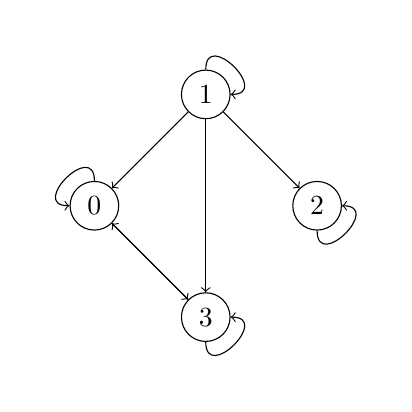
\begin{tikzpicture}[main/.style={draw,circle},node distance={2cm}]
                \node[main](0){$0$};
                \node[main](1)[above right of=0]{$1$};
                \node[main](2)[below right of=1]{$2$};
                \node[main](3)[below right of=0]{$3$};
                \draw[->](0) to [out=90,in=180,looseness=3] (0);
                \draw[->](0) -- (3);
                \draw[->](1) to [out=90,in=0,looseness=3] (1);
                \draw[->](1) -- (0);
                \draw[->](1) -- (2);
                \draw[->](1) -- (3);
                \draw[->](2) to [out=270,in=0,looseness=3] (2);
                \draw[->](3) -- (0);
                \draw[->](3) to [out=270,in=0,looseness=3] (3);
            \end{tikzpicture}
        \end{center}
        Hence the communication classes are $\left\lbrace 0,3 \right\rbrace, \left\lbrace 1 \right\rbrace, \left\lbrace 2 \right\rbrace$. Moreover, we note that
        \begin{equation*}
            d\left( 0 \right) = d\left( 1 \right) = d\left( 2 \right) = d\left( 3 \right) = 1,
        \end{equation*}
        since
        \begin{equation*}
            P{\left( 1 \right)}_{i,i} = P_{i,i} > 0
        \end{equation*}
        for all $i\in\left\lbrace 0,1,2,3 \right\rbrace$. Thus we conclude that the DTMC is aperiodic.
    \end{subproof}

    \ex Consider a DTMC with TPM
    \begin{equation*}
        P =
        \begin{bmatrix}
        	0 & 1 & 0 & 0 \\
        	0 & 0 & 1 & 0 \\
        	0 & 0 & 0 & 1 \\
        	\frac{1}{2} & 0 & \frac{1}{2} & 0 \\
        \end{bmatrix}.
    \end{equation*}
    Determine the period of each state.

    \begin{subproof}[Answer]
        The state transition diagram of the DTMC is the following.
        \begin{center}
            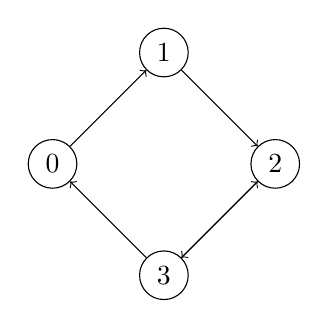
\begin{tikzpicture}[main/.style={draw,circle},node distance={2cm}]
                \node[main](0){$0$};
                \node[main](1)[above right of=0]{$1$};
                \node[main](2)[below right of=1]{$2$};
                \node[main](3)[below right of=0]{$3$};
                \draw[->](0) -- (1);
                \draw[->](1) -- (2);
                \draw[->](2) -- (3);
                \draw[->](3) -- (0);
                \draw[->](3) -- (2);
            \end{tikzpicture}
        \end{center}
        Note that it is clear from the diagram that
        \begin{equation*}
            P^{\left( n \right)}_{i,i}>0
        \end{equation*}
        only if $n$ is even for every $i\in\left\lbrace 0,1,2,3 \right\rbrace$. This means $d\left( i \right)\in\left\lbrace 2,4 \right\rbrace$ for all $i\in\left\lbrace 0,1,2,3 \right\rbrace$. For each $i\in\left\lbrace 0,1 \right\rbrace$, note that $P^{\left( 4 \right)}_{i,i}, P^{\left( 6 \right)}_{i,i} > 0$, so 
        \begin{equation*}
            d\left( 0 \right)=d\left( 1 \right)=2.
        \end{equation*}
        Moreover, for each $i\in\left\lbrace 2,3 \right\rbrace$, note that $P^{\left( 2 \right)}_{i,i}, P^{\left( 4 \right)}_{i,i}>0$, so
        \begin{equation*}
            d\left( 2 \right)=d\left( 3 \right)=2.
        \end{equation*}
        Thus $d\left( i \right)=2$ for all $i\in\left\lbrace 0,1,2,3 \right\rbrace$.
    \end{subproof}

    \ex Consider the DTMC with TPM
    \begin{equation*}
        P =
        \begin{bmatrix}
        	\frac{1}{2} & \frac{1}{2} & 0 & 0 \\
        	\frac{2}{3} & \frac{1}{3} & 0 & 0 \\
        	0 & 0 & 0 & 1 \\
        	0 & 0 & 1 & 0 \\
        \end{bmatrix}.
    \end{equation*}
    Find the communication classes of  this DTMC and determine the period of each state.

    \begin{subproof}[Answer]
        It is clear from the definition of $P$ that
        \begin{equation*}
            0\lra 1, 2\lra 3.
        \end{equation*}
        Also note that $P$ is a block diagonal matrix of the form
        \begin{equation*}
            P =
            \begin{bmatrix}
            	A & 0 \\
            	0 & B \\
            \end{bmatrix}
        \end{equation*}
        for some $A,B\in M_{2\times 2}(\R)$. This means
        \begin{equation*}
            P^n = 
            \begin{bmatrix} 
                A^n & 0 \\
                0 & B^n
            \end{bmatrix}
        \end{equation*}
        for every $n\in\N\cup\left\lbrace 0 \right\rbrace$, so the communication classes are $\left\lbrace 0,1 \right\rbrace, \left\lbrace 2,3 \right\rbrace$. Moreover, $P_{0,0}, P_{1,1}>0$, so $d\left( 0 \right)=d\left( 1 \right)=1$. Lastly, 
        \begin{equation*}
            B^n = 
            \begin{cases} 
                I_2 & \text{if $n$ is even}\\
                B & \text{if $n$ is odd}
            \end{cases},
        \end{equation*}
        so $d\left( 2 \right)=d\left( 3 \right)=2$.
    \end{subproof}

    \begin{prop}{Communication Preserves Periodicity}
        If $i,j$ are states of a DTMC that communicates, then $d\left( i \right)=d\left( j \right)$.
    \end{prop}

    \begin{proof}
        Since the result is clearly true when $i=j$, assume $i\neq j$. Since $i\lra j$, we know by definition that
        \begin{equation*}
            P^{\left( m \right)}_{j,i}, P^{\left( n \right)}_{i,j}>0
        \end{equation*}
        for some $n,m\in\N$. Moreover, since $i\lra j$ means $i\to j$ and $j\to i$, there exists $s\in\N$ such that
        \begin{equation*}
            P_{j,j}^{\left( s \right)}>0.
        \end{equation*}
        Note that 
        \begin{enumerate}
            \item $P_{i,i}^{\left( n+m \right)} \geq P^{\left( n \right)}_{i,j}P^{\left( m \right)}_{j,i} > 0$; and
            \item $P_{i,i}^{\left( n+m+s \right)} \geq P^{\left( n \right)}_{i,j}P^{\left( s \right)}_{j,j}P^{\left( m \right)}_{j,i} > 0$.
        \end{enumerate}
        (a), (b) implies that
        \begin{equation*}
            d\left( i \right)|s,
        \end{equation*}
        and in particular that
        \begin{equation*}
            d\left( i \right)|d\left( j \right).
        \end{equation*}
        By using the same argument, we also conclude that
        \begin{equation*}
            d\left( j \right)|d\left( i \right).
        \end{equation*}
        Thus $d\left( j \right)=d\left( i \right)$, as required.
    \end{proof}

    \ex Consider a DTMC with TPM
    \begin{equation*}
        P =
        \begin{bmatrix}
        	0 & \frac{1}{2} & \frac{1}{2} \\
        	\frac{1}{2} & 0 & \frac{1}{2} \\
        	\frac{1}{2} & \frac{1}{2} & 0 \\
        \end{bmatrix}.
    \end{equation*}
    Find the communication classes of this DTMC and determine the period of each state.

    \begin{subproof}[Answer]
        The following is the state transition diagram of the DTMC.
        \begin{center}
            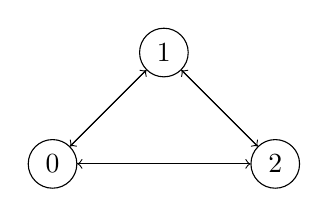
\begin{tikzpicture}[main/.style={draw,circle},node distance={2cm}]
                \node[main](0){$0$};
                \node[main](1)[above right of=0]{$1$};
                \node[main](2)[below right of=1]{$2$};
                \draw[->](0) -- (1);
                \draw[->](0) -- (2);
                \draw[->](1) -- (0);
                \draw[->](1) -- (2);
                \draw[->](2) -- (0);
                \draw[->](2) -- (1);
            \end{tikzpicture}
        \end{center}
        This means $\left\lbrace 0,1,2 \right\rbrace$ is the only communication class. Moreover, note that $0\to 1\to 0$ and $0\to 1\to 2\to 0$ are cycles of lengths $2,3$, respectively, so $d\left( 0 \right)=\gcd\left\lbrace 2,3,\ldots \right\rbrace=1$. It follows from Proposition 3.1 that
        \begin{equation*}
            d\left( 1 \right)=d\left( 2 \right)=d\left( 0 \right)=1. \eqqedsym
        \end{equation*}
    \end{subproof}

    \np As (EX 3.18) shows, it is possible to observe aperiodic behavior even though the main diagonal components of the TPM are zero. Generally, if $d\left( i \right)=k$, then it does not necessarily imply that $P^{\left( k \right)}_{i,i}>0$. Instead, it implies that if the DTMC is in state $i$ at time $0$, then it is impossible to observe the DTMC in state $i$ at time $n\in\N$ is $n$ is not a multiplie of $k$.

    \section{Transience and Recurrence}
    
    \np We desire to take a closer look at the likelihood of a DTMC beginning in some state of returning to that particular state. To that end, let us consider 
    the probability that, starting from state $i$, the first visit of the DTMC to state $j$ occurs at time $n\in\N$, denoted as $f^{\left( n \right)}_{i,j}$.

    \begin{notation}{$f^{\left( n \right)}_{i,j}$}{}
        Consider the setting of (3.20). We write $f^{\left( n \right)}_{i,j}$ to denote 
        \begin{equation*}
            f^{\left( n \right)}_{i,j} = \PP\left( X_n=j,\forall m\in\left\lbrace n-1,\ldots,1 \right\rbrace\left[ X_m\neq j \right]|X_0=i \right)
        \end{equation*}
        for all $i,j\in\N\cup\left\lbrace 0 \right\rbrace$.
    \end{notation}

    \noindent It is clear from Notation 3.10 that 
    \begin{equation*}
        f^{\left( 1 \right)}_{i,j} = \PP\left( X_1=j|X_0=i \right) = P_{i,j},
    \end{equation*}
    where $P$ is the TPM of the DTMC. For every $n\geq 2$, the determination of $f^{\left( n \right)}_{i,j}$ becomes more complicated, and so we desire to construct a procedure which will enable us to compute $f_{i,j}^{\left( n \right)}$. To do so, we consider the quantity $P^{\left( n \right)}_{i,j}$ and condition on the time that the first visit to state $j$ is made:
    \begin{flalign*}
        && P^{\left( n \right)}_{i,j} & = \PP\left( X_n=j|X_0=i \right) && \\ 
        && & = \sum^{n}_{k=1}\PP\left( X_n=j, \text{first visit to $j$ occurs at $k$}|X_0=i \right) && \\
        && & = \sum^{n}_{k=1}\PP\left( X_n=j, X_k=j,X_{k-1}\neq j,\ldots,X_1\neq j|X_0=i \right) && \\
        && & = \sum^{n}_{k=1}\PP\left( X_k=j,X_{k-1}\neq j,\ldots,X_1\neq j|X_0=j \right)\PP\left( X_n=j|X_k=j \right) && \text{by the Markov property} \\
        && & = \sum^{n}_{k=1}f^{\left( k \right)}_{i,j}P^{\left( n-k \right)}_{j,j}. && 
    \end{flalign*} 
    This means
    \begin{equation*}
        P^{\left( n \right)}_{i,j} 
        = f^{\left( n \right)}_{i,j}P^{\left( 0 \right)}_{j,j} + \sum^{n-1}_{k=1} f^{\left( k \right)}_{i,j}P^{\left( n-k \right)}_{j,j} = 
        = f^{\left( n \right)}_{i,j} + \sum^{n-1}_{k=1} f^{\left( k \right)}_{i,j}P^{\left( n-k \right)}_{j,j}.
    \end{equation*}
    Rearranging with respect to $f^{\left( n \right)}_{i,j}$ gives
    \begin{eqbox}[A Recursive Formula for $f^{\left( n \right)}_{i,j}$]
        \begin{equation}
            f^{\left( n \right)}_{i,j} = 
            P^{\left( n \right)}_{i,j} + \sum^{n-1}_{k=1} f^{\left( k \right)}_{i,j}P^{\left( n-k \right)}_{j,j}.
        \end{equation}
    \end{eqbox} 
    When $n\geq 2$, [3.6] yields a recursive means to compute $f^{\left( n \right)}_{i,j}$.

    \begin{notation}{$f_{i,j}$}{}
        Given a DTMC, let $f_{i,j}$ denote
        \begin{equation*}
            f_{i,j} = \PP\left( \exists n\in\N\left[ X_n=j \right]|X_0=i \right).
        \end{equation*}
    \end{notation}

    \noindent Note that
    \begin{flalign*}
        && f_{i,j} & = \sum^{\infty}_{k=1}\PP\left( \exists n\in\N\left[ X_n=j \right], X_k=j, X_{k-1}\neq j,\ldots,X_1\neq j|X_0=i \right) && \\ 
        && & = \sum^{\infty}_{k=1} \PP\left( X_k=j, X_{k-1}\neq j, \ldots, X_1\neq j|X_0=i \right) && \\
        && & = \sum^{\infty}_{k=1} f^{\left( k \right)}_{i,j} && \\
        && & \leq 1.
    \end{flalign*} 
    This leads to the following important concept in the study of Markov chains.

    \begin{definition}{Transient, Recurrent}{State}
        Given a state $i$ of a DTMC, we say $i$ is
        \begin{enumerate}
            \item \emph{transient} if $f_{i,i}<1$; and
            \item \emph{recurrent} if $f_{i,i}=1$.
        \end{enumerate}
    \end{definition}

    \np[Characterizing Transience and Recurrence]In what follows, we proceed to look at alternative ways of characterizing the notions of transience and recurrence. As such, let us first define $M_i$ be a random variable which counts the number of (future) times the DTMC visits state $i$, disregarding the possibility of starting in state $i$ at time $0$. If we assume that $f_{i,i}<1$, then the Markov property and stationary assumption imply that
    \begin{equation}
        \PP\left( M_i=k|X_0=i \right) = \left( \prod^{k}_{n=1}f_{i,i} \right)\left( 1-f_{i,i} \right)=f^k_{i,i}\left( 1-f_{i,i} \right)
    \end{equation}
    for every $k\in\N\cup\left\lbrace 0 \right\rbrace$, as  the DTMC will return to state $i$ $k$ times with probability $f_{i,i}$ and then never return with probability $1-f_{i,i}$. But note that [3.7] is the pmf of $\geodis_f\left( 1-f_{i,i} \right)$ (i.e. $M_i|\left( X_0=i \right)\sim\geodis_f\left( 1-f_{i,i} \right)$). This implies
    \begin{equation*}
        \EE\left( M_i|X_0=i \right) = \frac{1-\left( 1-f_{i,i} \right)}{1-f_{i,i}} = \frac{f_{i,i}}{1-f_{i,i}}
    \end{equation*}
    since $f_{i,i}<1$. On the other hand, if $f_{i,i}=1$, then $\PP\left( M_i>k|X_0=i \right)=1$ for all $k\in\N$, implying that
    \begin{equation*}
        \EE\left( M_i|X_0=i \right)=\infty.
    \end{equation*}
    To obtain another characterization, we may define a sequence of indicator random variables $\left( A_{n} \right)^{\infty}_{n=1}$ by
    \begin{equation*}
        A_n = 
        \begin{cases} 
            0 & \text{if $X_n\neq i$}\\
            1 & \text{if $X_n=i$}
        \end{cases}
    \end{equation*}
    for all $n\in\N$. With this definition,
    \begin{equation*}
        M_i = \sum^{\infty}_{n=1}A_n.
    \end{equation*}
    This means
    \begin{flalign*}
        && \EE\left( M_i|X_0=i \right)&=\EE\left( \sum^{\infty}_{n=1}A_n|X_0=i \right) = \sum^{\infty}_{n=1}\EE\left( A_n|X_0=i \right) && \\ 
        && & = \sum^{\infty}_{n=1} 0\cdot\PP\left( A_n=0|X_0=i \right)+1\cdot\PP\left( A_n=1|X_0=i \right) = \sum^{\infty}_{n=1}\PP\left( X_n=i|X_0=i \right) && \\
        && & =\sum^{\infty}_{n=1}P^{\left( n \right)}_{i,i}.
    \end{flalign*} 
    We summarize our characterizations into the following proposition.

    \clearpage
    \begin{prop}{Characterizations of Transience}
        Let $i$ be a state of a DTMC. The following are equivalent.\footnote{Of course, negations of (b), (c) are characterizations of recurrence.}
        \begin{enumerate}
            \item $i$ is transient.
            \item $\EE\left( M_i|X_0=i \right)$ is finite, where $M_i$ is the number of (future) times the DTMC visits state $i$.
            \item The series $\sum^{\infty}_{n=1}P^{\left( n \right)}_{i,i}$ is convergent.
        \end{enumerate}
    \end{prop}

    \noindent In other words, a transient state will only be visited \textit{finitely often}.

    \begin{prop}{Communication Preserves Recurrence}
        Let $i,j$ be states that communicate. Then $i$ is recurrent if and only if $j$ is recurrent.
    \end{prop}

    \begin{proof}
        It suffices to show that when $i$ is recurrent, then so is $j$. So assume that $i$ is recurrent. Since $i\lra j$, there exists $m,n\in\N\cup\left\lbrace 0 \right\rbrace$ such that 
        \begin{equation*}
            P_{i,j}^{\left( m \right)} , P^{\left( n \right)}_{j,i}>0.
        \end{equation*}
        Also, since $i$ is recurrent, we know that the series $\sum^{\infty}_{k=1}P^{\left( k \right)}_{i,i}$ is divergent. Now, note that
        \begin{equation*}
            P^{\left( n+k+m \right)}_{j,j} \geq P^{\left( n \right)}_{j,i}P^{\left( k \right)}_{i,i}P^{\left( m \right)}_{i,j} 
        \end{equation*}
        for every $k\in\N$. This means the series
        \begin{equation*}
            \sum^{\infty}_{l=n+m+1} P_{j,j}^{\left( l \right)} = \sum^{\infty}_{k=1} P_{j,j}^{\left( n+k+m \right)} = P^{\left( n \right)}_{j,i}P^{\left( m \right)}_{i,j}\sum^{\infty}_{k=1}P^{\left( k \right)}_{i,i}
        \end{equation*}
        is divergent, since $P^{\left( m \right)}_{i,j},P^{\left( n \right)}_{j,i}>0$, so $\sum^{\infty}_{l=1}P^{\left( l \right)}_{j,j}$ is also divergent. Thus $j$ is recurrent, as required.
    \end{proof}

    \begin{prop}{}
        If $i,j$ are states of a DTMC that communicates and $i$ is recurrent, then
        \begin{equation*}
            f_{i,j} = 1.
        \end{equation*}
    \end{prop}

    \begin{proof}
        We may assume $i\neq j$. Since $i\lra j$ and $i$ is recurrent, $j$ is recurrent by Proposition 3.3. This means $f_{j,j}=1$. To prove $f_{i,j}=1$, suppose $f_{i,j}<1$ for the sake of contradiction. Since $i\lra j$, let
        \begin{equation*}
            n_i = \min\left\lbrace n\in\N: P^{\left( n \right)}_{j,i}>0 \right\rbrace.
        \end{equation*}
        That is, each time the DTMC visits to state $j$, there is a nonzero probability $P^{\left( n_i \right)}_{j,i}>0$ of being in state $i$ $n_i$ time units later. Since we assumed $f_{i,j}<1$, then this means that the probability of returning to state $j$ after visiting $i$ in the future is not guaranteed, as $1-f_{i,j}>0$. Therefore, we have
        \begin{equation*}
            1-f_{j,j} = \PP\left( \forall n\in\N\left[ X_n\neq j \right]|X_0=j \right) \geq \underbrace{P^{\left( n_i \right)}_{j,i}}_{>0}\underbrace{\left( 1-f_{i,j} \right)}_{>0} > 0,
        \end{equation*}
        so $f_{j,j}<1$, which is our desired contradiction. Thus $f_{i,j}=1$, as required.
    \end{proof}

    \begin{prop}{}
        Every finite-state DTMC has at least one recurrent state.
    \end{prop}

    \begin{proof}
        We may assume that $\mS = \left\lbrace 0,\ldots,N \right\rbrace$ for some $N\in\N$ is the state space of the DTMC. Assume that every state is transient for the sake of contradiction. For each $i\in\mS$, since we assumed $i$ is transient, $f_{i,i}<1$. This means that, after a finite amount of time, $T_i$, state $i$ will not be visited again. Consequently, after a finite amount of time
        \begin{equation*}
            T = \max_{i\in\mS}T_i,
        \end{equation*}
        has gone by, none of the states will be visited ever again. However, the DTMC must be in some state after $T$ units of time, so we obtain a contradiction. Thus there is a recurrent state of the DTMC.
    \end{proof}

    \begin{cor}{}
        Every irreducible finite-state DTMC is recurrent.\footnote{We say a DTMC is \emph{recurrent} if every state is recurrent.}
    \end{cor}	

    \ex Consider the DTMC with TPM
    \begin{equation*}
        P = 
        \begin{bmatrix}
        	0 & 1 & 0 & 0 \\
        	0 & 0 & 1 & 0 \\
        	0 & 0 & 0 & 1 \\
        	0.5 & 0 & 0.5 & 0 \\
        \end{bmatrix}.
    \end{equation*}
    Determine whether each state is transient or recurrent.

    \begin{subproof}[Answer]
        From (EX 3.13), we know that the DTMC is irreducible. Thus by Corollary 3.5.1, every state of the DTMC is recurrent.
    \end{subproof}

    \begin{prop}{}
        Let $i,j$ be states of a DTMC. If $i$ is recurrent and $i\nlra j$, then $P^{\left( k \right)}_{i,j}=0$ for every $k\in\N$.
    \end{prop}

    \begin{proof}
        For the sake of contradiction, assume $P^{\left( k \right)}_{i,j}>0$ for some $k\in\N$. Choose
        \begin{equation*}
            k_i = \min\left\lbrace k\in\N: P^{\left( k \right)}_{i,j}>0 \right\rbrace.
        \end{equation*}
        Then
        \begin{equation}
            P^{\left( n \right)}_{j,i} = 0
        \end{equation}
        for every $n\in\N$, since otherwise $i\lra j$. However, this means the DTMC has a nonzero probability of at least $P^{\left( k_i \right)}_{i,j}$ of never returning to state $i$, by the minimality of $k_i$ and [3.8]. This is a contradiction, so we conclude that $P^{\left( k \right)}_{i,j}=0$ for all $k\in\N$.
    \end{proof}

    \ex Consider a DTMC with TPM
    \begin{equation*}
        P = 
        \begin{bmatrix}
        	\frac{1}{3} & \frac{2}{3} & 0 & 0 \\
        	\frac{1}{2} & \frac{1}{4} & \frac{1}{8} & \frac{1}{8} \\
        	0 & 0 & 1 & 0 \\
        	\frac{3}{4} & \frac{1}{4} & 0 & 0 \\
        \end{bmatrix}.
    \end{equation*}
    Determine whether each state is transient or recurrent.

    \begin{subproof}[Answer]
        From (EX 3.14), we know that $\left\lbrace 0,1,3 \right\rbrace, \left\lbrace 2 \right\rbrace$ are the communication classes of the DTMC. Now observe that $P^{\left( n \right)}_{2,2} = 1$ for every $n\in\N$, so the series
        \begin{equation*}
            \sum^{\infty}_{n=1}P^{\left( n \right)}_{2,2}
        \end{equation*}
        diverges. So $2$ is recurrent. Since $2\nlra j$ for every $j\in\left\lbrace 0,1,3 \right\rbrace$, it follows that $0,1,3$ are recurrent by Proposition 3.6.
    \end{subproof}

    \np As the above example demonstrates, \textit{once a DTMC enters a recurrent class of states, it can never leave that class}. For this reason, a recurrent class is often referred to as a \textit{closed} class.

    \ex Consider a DTMC with TPM
    \begin{equation*}
        P =
        \begin{bmatrix}
        	\frac{1}{4} & 0 & \frac{3}{4} & 0 \\
        	0 & \frac{1}{3} & 0 & \frac{2}{3} \\
        	0 & 1 & 0 & 0 \\
        	0 & \frac{2}{5} & 0 & \frac{3}{5} \\
        \end{bmatrix}.
    \end{equation*}
    Determine whether each state is transient or recurrent.

    \begin{subproof}[Answer]
        The following is the state transition diagram for the DTMC.
        \begin{center}
            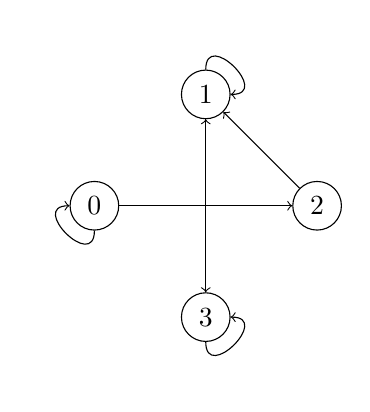
\begin{tikzpicture}[main/.style={draw,circle},node distance={2cm}]
                \node[main](0){$0$};
                \node[main](1)[above right of=0]{$1$};
                \node[main](2)[below right of=1]{$2$};
                \node[main](3)[below right of=0]{$3$};
                \draw[->](0) to [out=270,in=180,looseness=3] (0);
                \draw[->](0) -- (2);
                \draw[->](1) to [out=90,in=0,looseness=3] (1);
                \draw[->](1) -- (3);
                \draw[->](2) -- (1);
                \draw[->](3) to [out=270,in=0,looseness=3] (3);
                \draw[->](3) -- (1);
            \end{tikzpicture}
        \end{center}
        This means the communication classes of the DTMC are $\left\lbrace 0 \right\rbrace, \left\lbrace 1,3 \right\rbrace, \left\lbrace 2 \right\rbrace$. Now observe that
        \begin{equation*}
            \sum^{\infty}_{n=1}P^{\left( n \right)}_{0,0} = \sum^{\infty}_{n=1} \left( \frac{1}{4} \right)^n = \frac{1}{3},
        \end{equation*}
        so $0$ is transient. Moreover,
        \begin{equation*}
            \sum^{\infty}_{n=1}P^{\left( n \right)}_{2,2} = 0
        \end{equation*}
        clearly, so $2$ is transient. It follows from Proposition 3.3, 3.5 that $1,3$ are recurrent.
    \end{subproof}

    \section{Random Walk}

    \ex[Random Walk]Consider a DTMC $\left\lbrace X_n \right\rbrace^{}_{n\in\N\cup\left\lbrace 0 \right\rbrace}$ whose state space is $\Z$. Furthermore, suppose that the TPM $P$ for $\left\lbrace X_n \right\rbrace^{}_{n\in\N\cup\left\lbrace 0 \right\rbrace}$ satisfies
    \begin{flalign*}
        && P_{i,i-1} & = 1-p && \\
        && P_{i,i+1} & = p 
    \end{flalign*} 
    for all $i\in\Z$, where $p\in\left( 0,1 \right)$. As such, $X_n$ can be expressed as
    \begin{equation*}
        X_n = \sum^{n}_{k=0} Y_k,
    \end{equation*}
    where $\left\lbrace Y_k \right\rbrace^{\infty}_{k=0}$ is an independent collection of random variables with $Y_0=x_0$ and
    \begin{flalign*}
        && \PP\left( Y_k = -1 \right) & = 1-p && \\
        && \PP\left( Y_k=1 \right) & =p
    \end{flalign*} 
    for all $k\in\N$. Characterize the behavior of this DTMC in terms of its communication classes, periodicity, and recurrence.

    \begin{subproof}[Answer]
        Observe that the state transition diagram of the DTMC is the following.
        \begin{center}
            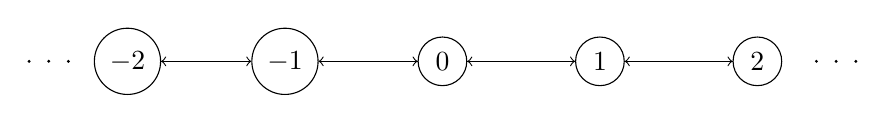
\begin{tikzpicture}[main/.style={draw,circle},node distance={2cm}]
                \node[main](0){$0$};
                \node[main](1)[right of=0]{$1$};
                \node[main](2)[right of=1]{$2$};
                \node[main](-1)[left of=0]{$-1$};
                \node[main](-2)[left of=-1]{$-2$};
                \draw[->](0) -- (1);
                \draw[->](0) -- (-1);
                \draw[->](1) -- (2);
                \draw[->](1) -- (0);
                \draw[->](2) -- (1);
                \draw[->](-1) -- (0);
                \draw[->](-1) -- (-2);
                \draw[->](-2) -- (-1);
                \draw[fill](4.75,0) circle (0.3pt);
                \draw[fill](5,0) circle (0.3pt);
                \draw[fill](5.25,0) circle (0.3pt);
                \draw[fill](-4.75,0) circle (0.3pt);
                \draw[fill](-5,0) circle (0.3pt);
                \draw[fill](-5.25,0) circle (0.3pt);
            \end{tikzpicture}
        \end{center}
        Since $p\in\left( 0,1 \right)$, all states communicate with each other, which means $\Z$ is the communication class of the DTMC, and the DTMC is irreducible. Furthermore, starting from state $0$, the DTMC cannot visit $0$ again in an odd number of transitions. On the other hand, $0\to 2\to 0$ is a cycle of length $2$. This means the period of $0$ is $2$. Since periodicity is a class property, it follows that
        \begin{equation*}
            d\left( i \right)=2
        \end{equation*}
        for all $i\in\Z$. Finally, to determine recurrence of state $0$, note that
        \begin{equation*}
            \sum^{\infty}_{m=1}P^{\left( m \right)}_{0,0} = \sum^{\infty}_{n=1}P^{\left( 2n \right)}_{0,0} = \sum^{\infty}_{n=1} \binom{2n}{n}p^n\left( 1-p \right)^n
        \end{equation*}
        since $P^{\left( m \right)}_{0,0}=0$ for all odd $m\in\N$. Now note that
        \begin{flalign*}
            && \lim_{n\to\infty} \frac{P^{\left( 2\left( n+1 \right) \right)}}{P^{\left( 2n \right)}}& =\lim_{n\to\infty} \frac{\binom{2n+2}{n+1}p^{\left( n+1 \right)}\left( 1-p \right)^{n+1}}{\binom{2n}{n}p^n\left( 1-p \right)^n} = \lim_{n\to\infty} \frac{\frac{\left( 2n+2 \right)!}{\left( n+1 \right)!\left( n+1 \right)!}p^{n+1}\left( 1-p \right)^{n+1}}{\frac{2n!}{n!n!}p^n\left( 1-p \right)^n} &&\\
            && & = \lim_{n\to\infty} \frac{\left( 2n+2 \right)\left( 2n+1 \right)}{\left( n+1 \right)\left( n+1 \right)} p\left( 1-p \right) = \lim_{n\to\infty} 4p\left( 1-p \right) = 4p\left( 1-p \right).
        \end{flalign*} 
        This means, when $p\neq \frac{1}{2}$,
        \begin{equation*}
            \lim_{n\to\infty} \frac{P^{\left( 2\left( n+1 \right) \right)}}{P^{\left( 2n \right)}} = 4p\left( 1-p \right)<1,
        \end{equation*}
        so the series $\sum^{\infty}_{n=1}P^{\left( 2n \right)}_{0,0}$ converges by the ratio test. In case $p=\frac{1}{2}$, 
        \begin{equation*}
            \lim_{n\to\infty} \frac{P^{\left( 2\left( n+1 \right) \right)}}{P^{\left( 2n \right)}} = 1,
        \end{equation*}
        so the ratio test is inconclusive. To determine what is happening when $p=\frac{1}{2}$, we consider an alternative approach. Recall that
        \begin{equation*}
            f_{i,j} = \PP\left( \exists n\in\N\left[ P_n=j \right]|X_0=i \right)
        \end{equation*}
        For convenience, let $q=1-p$. We condition on the state of the DTMC at time 1:
        \begin{flalign*}
            && f_{0,0} = & \,\,\PP\left( \exists n\in\N\left[ X_n=0 \right]|X_0=0 \right) && \\ 
            && = & \,\,\PP\left( X_1=-1|X_0=0 \right)\PP\left( \exists n\geq 2\left[ X_n=0 \right]|X_1=-1,X_0=0 \right) && \\
            && & + \PP\left( X_1=1|X_0=0 \right)\PP\left( \exists n\geq 2\left[ X_n=0 \right]|X_1=1,X_0=0 \right) && \\
            && = & \,\,\PP\left( X_1=-1|X_0=0 \right)\PP\left( \exists n\geq 2\left[ X_n=0 \right]|X_1=-1 \right) && \\
            && & + \PP\left( X_1=1|X_0=0 \right)\PP\left( \exists n\geq 2\left[ X_n=0 \right]|X_1=1 \right) && \text{by the Markov property}\\
            && = & \,\,qf_{-1,0}+pf_{1,0}.
        \end{flalign*} 
        If we let $E$ represent the event that the DTMC ever makes a future visit to state $0$, then
        \begin{equation*}
            E = \bigcup^{\infty}_{i=1} \left\lbrace X_i = 0 \right\rbrace.
        \end{equation*}
        So
        \begin{flalign*}
            && f_{1,0} & = \PP\left( F|X_1=0 \right) && \\
            && = &\,\,\PP\left( F\cap \left\lbrace X_1=0 \right\rbrace | X_0=1\right) + \PP\left( F\cap\left\lbrace X_1=2 \right\rbrace|X_0=1 \right) && \\
            && = &\,\,\underbrace{\PP\left( F|X_1=0,X_0=1 \right)}_{=1}\PP\left( X_1=0|X_0=1 \right) && \\
            && & + \PP\left( F|X_1=2,X_0=1 \right)\PP\left( X_1=2|X_0=1 \right) && \\
            && = &\,\,\PP\left( X_1=0|X_0=1 \right) + \PP\left( F|X_1=2 \right)\PP\left( X_1=2|X_0=1 \right) && \substack{\text{by the Markov}\\\text{property}}\\
            && = &\,\,q + p\PP\left( E|X_1=2 \right) && \\
            && = &\,\,q + p\PP\left( \bigcup^{\infty}_{i=2}\left\lbrace X_i=0 \right\rbrace\union\left\lbrace X_1=0 \right\rbrace|X_1=2 \right) && \\
            && = &\,\,q + p\PP\left( \bigcup^{\infty}_{i=2}\left\lbrace X_i=0 \right\rbrace|X_1=2 \right) && \substack{\text{since}\\\PP\left( X_1=0|X_1=2 \right)=0}\\
            && = &\,\,q + p\PP\left( E | X_0=2 \right) && \substack{\text{by the stationary}\\\text{assumption}} \\
            && = &\,\,q + pf_{2,0}.
        \end{flalign*} 
        Furthermore, it is clear from the defintion of the DTMC that
        \begin{equation*}
            f_{2,0} = f_{2,1}f_{1,0} = f_{1,0}^{2},
        \end{equation*}
        where the last equality holds by the stationary assumption. Hence we obtain that
        \begin{equation*}
            f_{1,0} = \left( 1-p \right)+pf_{1,0}^{2},
        \end{equation*}
        and by rearranging in terms of $f_{1,0}$ gives
        \begin{equation*}
            pf^{2}_{1,0} - f_{1,0} + 1 - p = 0.
        \end{equation*}
        By applying the quadratic formula,
        \begin{equation}
            f_{1,0} = \frac{1\pm\sqrt{1-4p\left( 1-p \right)}}{2p} = 1,
        \end{equation}
        since $p=\frac{1}{2}$. By symmetry, $f_{-1,0} = 1$. This means
        \begin{equation*}
            f_{0,0} = \left( 1-p \right)f_{-1,0}+pf_{1,0} = \frac{1}{2} + \frac{1}{2} = 1,
        \end{equation*}
        so $0$ is recurrent. Thus every state of the DTMC is recurrent, since recurrence is a class property.
    \end{subproof}

    \noindent Note that, when $p\neq \frac{1}{2}$, the first equality in [3.9] yields
    \begin{equation*}
        f_{1,0} \in \left\lbrace \frac{1+\left| 2p-1 \right|}{2p}, \frac{1-\left| 2p-1 \right|}{2p} \right\rbrace.
    \end{equation*}
    We may assume $p<\frac{1}{2}$. This means $2p-1<0$, so
    \begin{flalign*}
        && \frac{1-\left( 1-2p \right)}{2p} & = 1 && \\
        && \frac{1+\left( 1-2p \right)}{2p} & > 1 && 
    \end{flalign*} 
    which means $f_{1,0} = 1$, since a probability cannot be greater than $1$. In other words,
    \begin{equation*}
        f_{1,0} = \frac{1-\left| 1-2p \right|}{2p}.
    \end{equation*}
    Moreover, it can be shown that
    \begin{equation*}
        f_{-1,0} = \frac{1-\left| 1-2p \right|}{2\left( 1-p \right)}.
    \end{equation*}
    Thus we obtain that
    \begin{equation*}
        f_{0,0} = \left( 1-p \right) \frac{1-\left| 1-2p \right|}{2\left( 1-p \right)} + p \frac{1-\left( 1-2p \right)}{2p} = 1-\frac{1}{2} \left( 2-4p \right) = 1-\left( 1-2p \right) = 2p < 1
    \end{equation*}
    when $p<\frac{1}{2}$, which is consistent with our earlier finding that the DTMC is transient when $p\neq \frac{1}{2}$. In general, we have the following formula:
    \begin{eqbox}[General Formula for $f_{0,0}$ of a Random Walk]
        \begin{equation}
            f_{0,0} = 2\min\left\lbrace p,1-p \right\rbrace.
        \end{equation}
    \end{eqbox} 































    
    
    
    
    
    
    
    
    
    
    

\end{document}
